%*********************************************************************
% Maintained by 
%    wjw (wjw152908@gmail.com)
%    zhy (zhaohanyu426@gmail.com)
% 
% 2024/04/30 v0.1
% Notice & Disclaimer:
%   1. 本模版基于'School of Computing and Data Science(SCDS % )'所提供的FYP Thesis Template 31 March 2024.docx'模版制作。
%   2. 由于各院系要求有略微不同,使用本模版前请先和自己的导师和系FYP % coordinator沟通。
%   2. 本模版参考文献引用格式为APA格式,若不同院系有各自要求请自行调 % 整。
%   3. 修改、使用、发布本文档请遵循 LaTeX Project Public License
%   4. 由于Latex格式限制,目录部分(Table of Content)和学校给的模版  % 文档有所不同。请按照自己的需求进行调整。
%   5. 请使用最新版本的模板,打印前检查输入信息与学院要求是否一致
%*********************************************************



\documentclass[12pt, a4paper]{report}
\usepackage{fontspec}
\usepackage{geometry}
\usepackage{apacite}
\usepackage{titlesec}
\usepackage{graphicx}
\usepackage{afterpage}
\usepackage{lipsum}
\usepackage{ragged2e}
\usepackage{titletoc}       %目录格式宏
\usepackage{multirow}

%编辑目录格式

% 定制chapter部分的格式
\titleformat{\chapter}[display]
{\small\bfseries\centering} % 字体和样式
{\chaptertitlename} % 标题与数字格式
{50pt} % 章节与标题之间的距离
{\small} % 标题的大小

\titlespacing*{\chapter}{0pt}{0pt}{0pt} % 调整章节标题的间距



% 定制section部分的格式
\titlecontents{section}[2em]
{\bfseries}% 设置部分标题为粗体
{\uppercase\thecontentslabel.}
{}
{\titlerule*[0.5pc]{}\bfseries\thecontentspage}% 设置页码为粗体和较大的字体


% 定制subsection部分的格式
\titlecontents{subsection}
[2em]
{\small}% 设置部分标题为较小的字体
{\thecontentslabel. }
{}
{\titlerule*[0.5pc]{}\bfseries\thecontentspage}

% \renewcommand{\contentsname}{
	%     \centering\small\uppercase\textbf{Table of Contents}
	% } 
% \renewcommand{\contentsname}{
	%     \centering\small\uppercase\textbf{Table of Contents}
	% } 

\newfontfamily\titlefont{Arial}[Scale=1.2] %首页字号为小二/18pt 已设置好
\newfontfamily\theistitle{Times New Roman}[Scale=1.3]
\newfontfamily\fypsentence{Times New Roman}[Scale=1.1]
\renewcommand{\contentsname}{Table of Contents}

\renewcommand{\baselinestretch}{1.3} % 设置行间距为 1.3倍
\geometry{
	top=2.5cm,
	bottom=2.5cm,
	left=4cm,
	right=2.5cm
}



\begin{document}
	\begin{center}		
		\titlefont
		\uppercase{\textbf{\large{\\ \vspace{2cm} AN EXPLORATION OF THE EFFECTS OF MOODS IN ATTITUDE JUDGEMENTS(Thesis title)}}}            %论文题目
		
		\vspace{7cm}
		
		\textbf{\large YVONNE CAROLINE(sample name)}   %姓名
		
		\vspace{10cm}
		
		\uppercase{\textbf{\large{Xiamen University Malaysia}}}
		\\
		\vspace{0.5cm}
		\uppercase{\textbf{\large{2024}}}
	\end{center}
	%cover页结束
	
	
	
	
	
	
	
	
	
	
	
	
	
	
	
	
	
	
	
	
	
	
	
	\newpage
	\centering
	
\includegraphics[width=14.53cm,height=3cm]{XMUM LOGO.png}
	
	\vspace{2cm}
	
	{\centering
		\fypsentence
		FINAL YEAR PROJECT REPORT
		\par}
	
	\vspace{3.5cm}
	{\centering
		\theistitle
		\textbf{CADMIUM BIOSORPTION USING FREE 
			AND IMMOBILISED BIOMASS OF ASPERGILLUS AWAMORI
		}\par}  %填写毕业论文的题目
	
	\vspace{4cm}
	
	\begin{table}[ht]
		\centering
		\begin{tabular}{lll}
			NAME OF STUDENT & : & WU JUNWEI             %名字
			\\
			STUDENT ID      & : & MAT1909415            %学号
			\\
			SCHOOL/ FACULTY & : & \begin{tabular}[c]{@{}l@{}}SCHOOL OF COMPUTING AND DATA \\ SCIENCE\end{tabular}                                 \\
			%学院名 若超出页面边界请手动换行
			PROGRAMME       & : & \begin{tabular}[c]{@{}l@{}}BACHELOR OF ENGINEERING IN \\ COMPUTER SCIENCE AND                                 %专业名 若超出页面边界请手动换行
				\\ TECHNOLOGY (HONOURS)\end{tabular} \\
			INTAKE          & : & 2021/02                                                                                                          \\
			SUPERVISOR      & : & Goh Sim Kuan          %导师名字
			\\
			&   & Assistant Professor   %导师的职称                                  
		\end{tabular}
	\end{table}
	
	\vspace{2cm}
	
	{\centering
		\textbf{AUGUST 2024}
		\par}
	
	
	
	
	
	
	
	
	
	
	
	
	
	
	
	
	
	
	\newpage
	\addcontentsline{toc}{chapter}{1  DECLARATION}
	
	{\centering
		\textbf{DECLARATION}
	}
	% \section*{\centering DECLARATION}
	
	
	
	
	\vspace{4cm}
	\begin{justify}
		{
			
			I hereby declare that this project report is based on my original work except for citations and quotations which have been duly acknowledged. I also declare that it has not been previously and concurrently submitted for any other degree or award at Xiamen University Malaysia or other institutions.
			
		}
	\end{justify}
	\vspace{4cm}
	
	\begin{RaggedRight}
		Signature\ \ : \_\_\_\_\_\_\_\_\_\_\_\_\_\_\_\_\_\_\_\_\
		
		Name \ \ \ \ : \_\_\_\_\_\_\_\_\_\_\_\_\_\_\_\_\_\_\_\_\_
		
		ID No.\ \ \ \ : \_\_\_\_\_\_\_\_\_\_\_\_\_\_\_\_\_\_\_\_\_
		
		Date\ \ \ \ : \_\_\_\_\_\_\_\_\_\_\_\_\_\_\_\_\_\_\_\_\_\_
		
	\end{RaggedRight}
	
	
	
	
	
	
	
	
	
	
	
	
	
	
	\newpage
	\addcontentsline{toc}{chapter}{2  APPROVAL FOR SUBMISSION}
	\textbf{APPROVAL FOR SUBMISSION}
	
	
	\vspace{4cm}
	
	\begin{justify}
		{
			
			I certify that this project report entitled “\textbf{TITLE TO BE THE SAME AS FRONT COVER, CAPITAL LETTER, BOLD}” that was prepared by STUDENT’S NAME has met the required standard for submission in partial fulfillment of the requirements for the award of Bachelor of Engineering in Computer Science and Technology (Honours) at Xiamen University Malaysia.
			
			\vspace{3cm}
			\RaggedRight
			Approved by,
			\vspace{4cm}
			
		}
	\end{justify}
	\begin{RaggedRight}
		Signature\ \ \ \ \ \ : \_\_\_\_\_\_\_\_\_\_\_\_\_\_\_\_\_\
		\\
		Supervisor \ \ \ : Dr.Goh Sim Kuan          %修改成导师名字
		\\
		Date\ \ \ \ \ \ \ \ \ \ \ \  : \_\_\_\_\_\_\_\_\_\_\_\_\_\_\_\_\_
		\\
		
	\end{RaggedRight}
	
	
	
	
	
	
	
	
	
	
	
	
	
	\newpage
	\bigskip
	
	\begin{justify}
		{
			\vspace*{4cm}
			The copyright of this report belongs to the author under the terms of Xiamen University Malaysia copyright policy. Due acknowledgment shall always be made of the use of any material contained in, or derived from, this project report/thesis.
			
			\vspace{2cm}
			©2024, Name of Candidate.      %替换成自己名字
			All right reserved.
		}
		
	\end{justify}
	
	
	
	
	
	
	
	
	
	
	
	
	
	
	
	
	
	\newpage
	\addcontentsline{toc}{chapter}{3 ACKNOWLEDGEMENTS}
	\textbf{ACKNOWLEDGEMENTS}     %致谢部分,自行修改
	
	\vspace{3cm}
	\begin{justify}
		{
			I would like to thank all who have contributed to the successful completion of this project. I would like to express my gratitude to my research supervisor, Prof. Dr. XXXXX for his invaluable advice, guidance and his enormous patience throughout the development of the research.
			
			\vspace{0.5cm}
			
			\noindent In addition, I would also like to express my gratitude to my loving parents and friends who have helped and given me encouragement.
		}
	\end{justify}
	
	
	
	
	
	
	
	
	
	
	
	
	
	
	
	
	
	
	
	
	
	\newpage
	\addcontentsline{toc}{chapter}{4 ABSTRACT}
	\textbf{ABSTRACT} %摘要
	% \section*{\centering ABSTRACT}
	
	\begin{justify}
		{
			The abstract should be brief, not more than \textbf{500 words}. (As required by CST department)
			
			Keywords should indicate the novelty and relevant major points of the project undertaken. A maximum of \textbf{five (5) keywords} could be listed below the abstract (optional). (As required by CST department)
			
			
		}
	\end{justify}
	
	
	
	
	
	
	
	
	
	
	
	
	
	
	
	
	
	
	\newpage
	%生成目录
	\tableofcontents

	%\chapter{} %不需要填写内容
	
	
	
	
	
	
	
	
	
	
	
	
	
	\setcounter{chapter}{4}
	\chapter{\textbf{INTRODUCTION}}{
		% \addcontentsline{toc}{chapter}{CHAPTER} %目录中的名字 如CHAPTER、REFERENCES、APPENDIX

		\begin{flushleft}
			\section{Background}{
				% Background contents here
				Spacing between title of subsection and first line of text is 1.5 lines. The first paragraph in a subsection should align with left margin.
				Spacing between last line of text and the next subsection title is 1.5 lines.
			}
		\end{flushleft}
		
		\begin{flushleft}
			\section{Aims and Objectives}{
				% Aims and Objectives contents here
			}
		\end{flushleft}
		
		\begin{flushleft}
			\section{Thesis Content}{
				There is no restriction on the total number of chapters in a project report/ thesis. The number of chapters differs according to the field of study conducted by the candidate whether it is science-based or social-science-based. However, the content of the chapters may differ according to the candidate's research or conventions of individual School/ Faculty.
				
				The body of the Project Report/ Thesis must be written in paragraphs. There must be continuity or logical flow among paragraphs. Long paragraphs are advised to be avoided.
				
				Generally, a basic structure for the project report/ thesis is as below:
				
				•	Introduction
				
				•	Literature Review
				
				•	Research Methodology
				
				•	Results
				
				•	Discussion
				
				•	Conclusion and Recommendation
				
				•	References
				
				The level of English writing must be appropriate to the level of the Bachelor’s degree. Attention should be paid to correct spelling, grammar, punctuation, sentence structure and clarity of style.
				
				Normally, no first person references (e.g. I, we, us) shall appear in the report. If self-reference is required, reference may be made to “the author” or “this study”. Exceptions are acceptable in the conclusion section, where personal comments may be appropriate.
			}
		\end{flushleft}
	}
		
		
		
		
		
		
		
		
		
		
		
		
		
		
		
		
		
		
		
		\setcounter{chapter}{5}
		\setcounter{section}{0}
		\chapter{\textbf{LITERATURE REVIEW}}{
			\begin{flushleft}
				\section{Background}{
					A literature review is a description of the literature relevant to a particular field or topic of study. It consists of a critically written and comprehensive account of the published works on a topic by accredited scholars and researchers. A critical literature review is a critical assessment of the relevant literature. It is directly related to the research, providing information on theories, models, materials and techniques used in the research. The literature review should be comprehensive and include recent publications which are relevant to the research.
					
					The literature review should not be just a compilation or reproduction of the works of others. It requires the student to examine and comment critically on the literature relevant to the student’s area of research. Students should be aware of that getting hold of the right material is only a small part of the research process, but being able to put ideas, information, data and arguments together in an integrated and coherent manner makes the difference between success and failure.
					
					The literature review should clearly indicate what diversity of views exist among the authors in this area of study, and the student should show how and where his/her research fits in.
				}
				\section{Submission}{
					The minimum word limit for the Project Report/ Thesis, excluding tables and figures, and references is 10,000 words and must not exceed 30,000 words. However, the word limit may differ in each individual school/ faculty, academy, institute or center with its own additional requirements.
				}
				
				\section{Table Formatting}{
					% put your table here
					The tables should be arranged according to the chapters. The numbering system is according to the chapter, for e.g.: tables in Chapter 1 are numbered sequentially: Table 1.1, Table 1.2 and so on.
					
					\begin{table}[t]
						\caption{Technical Specification of Force Sensing Resistor}
						\centering
						\begin{tabular}{|c|c|}
							\hline
							Item &  Descriptions \\
							
							\hline
							&   \\
							\hline
							&   \\
							\hline
						\end{tabular}
						\label{tab:my_label}
					\end{table}
				}
				
				\section{Figure Formatting}{
					% put your figure here 
					Figures include diagrams, photographs, drawings, graphs, charts and maps. The figures should be arranged according to the chapters. For example, figures in Chapter 1 are numbered sequentially: Figure 1.1, Figure 1.2 and so on.

					\begin{figure}
						\centering
						\scalebox{0.5}{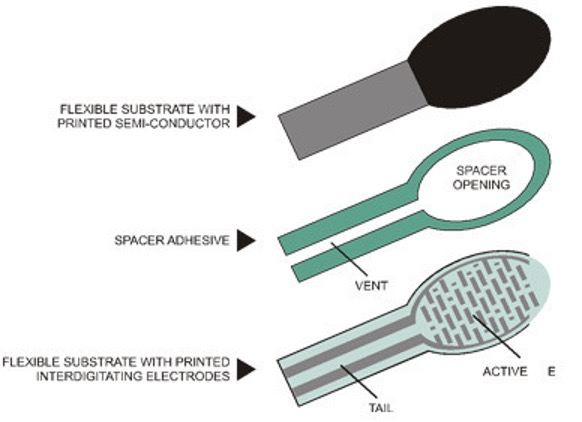
\includegraphics{figure_example.jpg}}
						\caption{Force Sensing Resistor}
						\label{fig:enter-label}
					\end{figure}
					
				}
			\end{flushleft}
			
		}
		
		
		
		
		
		
		
		
		
		\setcounter{chapter}{6}
        \setcounter{section}{0}
		\chapter{\textbf{RESEARCH METHODLOGY}}{
			\begin{flushleft}
				\section{Background}{
					This chapter describes and explains the materials as well as the research methodology used in the study. The sub-topics for this chapter include the key research questions, the research design, and the research procedures adopted. It may also, where appropriate, indicate sampling methods, research instruments and statistical methods employed. The purpose is to inform the reader on the methods used to collect the data and generate the findings reported.
				}
			\end{flushleft}
		}
		
		
		
		
		
		
		
		
		
		\setcounter{chapter}{7}
		\setcounter{section}{0}
		\chapter{ \textbf{RESULT AND DISCUSSION}}{
			\begin{flushleft}
				\section{Background}{
					% backgroud here
				}
		
				\section{Results}{
					Section 4.2 explains the results that are commonly presented in the form of text, figures and tables, along with data analysis
				}
				\section{Discussion}{
					Section 4.3 contains the interpretation of the results. Findings of the research should be compared and contrasted with those of previous studies presented in the literature review. The purpose of this chapter is to discuss the findings and the outcomes of the research in relation to the results that have been obtained
				}
				
				\end{flushleft}
			}
			
			
			\setcounter{chapter}{8}
			\setcounter{section}{0}
			
			
			
			
			
			
			
			
			
			
			
			
			
			
			
			
			
			\chapter{\textbf{CONCLUSION}}{
				\begin{flushleft}
				\section{Background}{
					In this chapter, findings are summarized and their implications are discussed. This section may include suggestions for future work
				}
				\end{flushleft}
	
			\section{Methods}{
				Details about the methods used.
				Attention mask is import \cite{DBLP:journals/corr/VaswaniSPUJGKP17}, and Literate Programming is also a serious part of it \cite{knuth:1984}. %\cite(bib代号) 自动引用
		
				\subsection{Algorithm A}{
					Description of Algorithm A.
				}
				
				\subsection{Algorithm B}{
					Description of Algorithm B.
				}
			}
			
			\section{Results}{
				Presentation of results.
			}
		
	}
			
			
			
			
			
		%APA 
		\bibliographystyle{apalike}
		\bibliography{reference.bib}
			
			
			
		
	\end{document}
	
